\documentclass[aspectratio=169,
hyperref={colorlinks,urlcolor=blue}
]{beamer}


%\usetheme{Pittsburgh}
\usetheme{default}
\usepackage{colortbl}%colored tables
%For using helvetica font:
\usepackage[scaled]{helvet}
\usepackage[T1]{fontenc}
\renewcommand\familydefault{\sfdefault}
\urlstyle{same} %sets the fonts for urls
\usepackage{pdfpages}
\usepackage{siunitx}
\usepackage{caption}
\usepackage{pifont}%for dings
\usepackage{pgfplots}%for 3d plotting
\pgfplotsset{compat = newest}
\usepackage{mathtools}%box in align env \Aboxed
\usepackage[american,smartlabels]{circuitikz}%for drawing circuits
\usepackage{multimedia}
\usepackage{animate}
\usepackage{xcolor}


\usetikzlibrary{arrows}
\usetikzlibrary {3d} 
\usetikzlibrary{decorations.markings, math}
\usetikzlibrary{intersections, pgfplots.fillbetween}
\usetikzlibrary {shapes.geometric} 


%\definecolor{myblue}{RGB}{5, 34, 150}
\definecolor{myblue2}{RGB}{5, 34, 150}
\definecolor{myblue}{RGB}{0,36,82}
\definecolor{myred}{RGB}{207, 2, 13}
\definecolor{mygreen}{RGB}{0, 158, 11}
\definecolor{myyellow}{RGB}{220,220,0}
\definecolor{qblue}{RGB}{0,36,82}
\definecolor{qgold}{RGB}{250,189,15}
\definecolor{qred}{RGB}{185,14,49}
\definecolor{cblue}{rgb}{0.13, 0.67, 0.8}
\definecolor{corange}{rgb}{0.8, 0.34, 0.0}
\definecolor{cpurple}{rgb}{0.54, 0.29, 0.42}

%%%%%%%%%%%% General settings
\setbeamercolor{frametitle}{fg=black}
\setbeamercolor{title}{fg=black}
\setbeamercolor{author}{fg=myblue2}

\beamertemplatenavigationsymbolsempty %no navigation controls at bottom of slides
%\setbeamertemplate{footline}[frame number]
\usefonttheme{professionalfonts} 
\setbeamerfont{title}{series=\bfseries,parent=structure}
\setbeamerfont{frametitle}{series=\bfseries,parent=structure}

%%%%%%%%%%%%Lists
\setbeamertemplate{itemize item}[circle] %{\color{myblue}$\circ$}
\setbeamertemplate{itemize subitem}{\color{myblue2}$\circ$}
\setbeamertemplate{itemize subsubitem}{\color{myblue2}$\cdot$}
\setbeamercolor{itemize item}{bg=myblue2,fg=myblue2}
\setbeamercolor{enumerate item}{bg=myblue2,fg=myblue2}
%%%%%%%%%%%%%%%%%%%%%%%%%%%%

%%%%%%%%%%%%Blocks
\setbeamertemplate{blocks}[rounded]
%Default block
\setbeamercolor{block title}{bg=myblue2, fg=white}
\setbeamercolor{block body}{bg=myblue2!10}
\setbeamerfont{block body}{size=\scriptsize}
\setbeamerfont{block title}{size=\scriptsize}
%Alert block
\setbeamercolor{block title alerted}{bg= myblue2, fg=white}
\setbeamercolor{block body alerted}{bg=myblue2!10}
\setbeamerfont{block body alerted}{size=\scriptsize}
\setbeamerfont{block title alerted}{size=\scriptsize}
%example block
\setbeamercolor{block title example}{bg=mygreen, fg=white}
\setbeamercolor{block body example}{bg=mygreen!10}
\setbeamerfont{block body example}{size=\scriptsize}
\setbeamerfont{block title example}{size=\scriptsize}
%%%%%%%%%%%%%%%%55


%%%%%%%%%%%%Figures and captions
\captionsetup{font=scriptsize,labelfont=scriptsize}
%\setbeamertemplate{caption}{\raggedright\insertcaption\par}
\newenvironment{capfig}[3]{\begin{figure}\includegraphics[width=#1\textwidth]{#2}\caption*{\textit{#3}}\end{figure}}{}

%\makeatother
%\setbeamertemplate{footline}
%{
%  \leavevmode%
%  \hbox{%
%  \begin{beamercolorbox}[wd=.4\paperwidth,ht=2.25ex,dp=1ex,center]{author in head/foot}%
%    \usebeamerfont{author in head/foot}\insertshortauthor
%  \end{beamercolorbox}%
%  \begin{beamercolorbox}[wd=.6\paperwidth,ht=2.25ex,dp=1ex,center]{title in head/foot}%
%    \usebeamerfont{title in head/foot}\insertshorttitle\hspace*{3em}
%    \insertframenumber{} / \inserttotalframenumber\hspace*{1ex}
%  \end{beamercolorbox}
%  }%
%  \vskip0pt%
%}
%\makeatletter

\makeatother
\setbeamertemplate{footline}
{
  \leavevmode%
  \hbox{%
\begin{beamercolorbox}[wd=.27\paperwidth,ht=2.25ex,dp=1ex,center]{author in head/foot}%
    \color{black}{\insertinstitute}
\end{beamercolorbox}
  \begin{beamercolorbox}[wd=.27\paperwidth,ht=2.25ex,dp=1ex,center]{author in head/foot}%
    \color{black}{\inserttitle}
  \end{beamercolorbox}%
  \begin{beamercolorbox}[wd=.27\paperwidth,ht=2.25ex,dp=1ex,center]{title in head/foot}%
    \color{black}{\insertshortauthor}
  \end{beamercolorbox}
  \begin{beamercolorbox}[wd=.27\paperwidth,ht=2.25ex,dp=1ex,center]{title in head/foot}%
    \hspace{.28\paperwidth}\color{black} \insertframenumber{} / \inserttotalframenumber\hspace*{1ex}
  \end{beamercolorbox}
  }%
  \vskip0pt%
}
\makeatletter

\setbeamertemplate{title page}
{
  \begin{tikzpicture}[remember picture,overlay]
    \def\barh{4}%15
  
    \draw[color=myblue2,line width=\barh] ([yshift=-0.5*\barh]current page.north west) -- ([yshift=-0.5*\barh,xshift=-0.67\paperwidth]current page.north east);
    \draw[color=myblue2,line width=\barh] ([yshift=-0.5*\barh,xshift=-0.67\paperwidth]current page.north east) -- ([yshift=-0.5*\barh,xshift=-0.34\paperwidth]current page.north east);
    \draw[color=myblue2,line width=\barh] ([yshift=-0.5*\barh,xshift=-0.34\paperwidth]current page.north east) -- ([yshift=-0.5*\barh]current page.north east); 
  
    \draw[color=myblue2,line width=\barh] ([yshift=0.5*\barh]current page.south west) -- ([yshift=0.5*\barh,xshift=-0.67\paperwidth]current page.south east);
    \draw[color=myblue2,line width=\barh] ([yshift=0.5*\barh,xshift=-0.67\paperwidth]current page.south east) -- ([yshift=0.5*\barh,xshift=-0.34\paperwidth]current page.south east);
    \draw[color=myblue2,line width=\barh] ([yshift=0.5*\barh,xshift=-0.34\paperwidth]current page.south east) -- ([yshift=0.5*\barh]current page.south east);
    %\node[left] at (current page.east) {
    %
\includegraphics[scale=0.1]{figures/coverpage}
    %};
  \end{tikzpicture}
  
  \usebeamerfont{title}\usebeamercolor[fg]{title}\inserttitle\par
  \usebeamerfont{subtitle}\usebeamercolor[fg]{subtitle}\insertsubtitle\par
  \vspace{2cm}
  \usebeamerfont{author}\usebeamercolor[fg]{author}\insertauthor\par
  \usebeamerfont{institute}\usebeamercolor[fg]{author}\insertinstitute\par
  \usebeamercolor[fg]{author}\par
  \usebeamercolor[fg]{titlegraphic}\inserttitlegraphic

} 

\setbeamertemplate{frametitle}{%
    \nointerlineskip%
        \par\hspace*{-\dimexpr0.5\paperwidth-0.5\textwidth}\textcolor{myblue2}{\rule{0.33\paperwidth}{6pt}}\textcolor{myblue2}{\rule{0.33\paperwidth}{6pt}}\textcolor{myblue2}{\rule{0.34\paperwidth}{6pt}} 
    \begin{beamercolorbox}[wd=\paperwidth,ht=0.75cm,dp=0.6ex]{frametitle}
        \hspace*{0.5cm}\strut\usebeamerfont{frametitle}\insertframetitle\strut
        %\hrule
    \end{beamercolorbox}%
    %%Line below:
%\par\hspace*{-\dimexpr0.5\paperwidth-0.5\textwidth}\textcolor{myblue}{\rule{\paperwidth}{0.4pt}}
     % <-- calculation of left margin width + rule
     %\textcolor{red}{\noindent\rule{\paperwidth}{2pt}}
}


%%%%%%%%%%%%Frame templates

%Slide with title
\newenvironment{titleframe}[1]
{\begin{frame}\frametitle{#1}\end{frame}}
{}

%Slide with title and itemize list:
\newenvironment{bulletframe}[1]
{\begin{frame}{#1} \itemize}
{\enditemize \end{frame}}

%Slide with two columns 50/50
\newenvironment{twocolframe}[3]
{\begin{frame}{#1}
 \begin{columns}[T]
 \column{0.5\textwidth}#2
 \column{0.5\textwidth}#3
 \end{columns}\end{frame}}{}

%Slide with two columns 60/40 <<<<<<<<<<<<<<<<<<<<<<  This one!
\newenvironment{twocolframesf}[3]
{\begin{frame}{#1}
 \begin{columns}[T]
 \column{0.6\textwidth}#2
 \column{0.4\textwidth}#3
 \end{columns}\end{frame}}{}
 
%Slide with two columns 70/30
\newenvironment{twocolframest}[3]
{\begin{frame}{#1}
 \begin{columns}[T] 
 \column{0.7\textwidth}#2
 \column{0.3\textwidth}#3
 \end{columns}\end{frame}}{} 
 
%Slide with two columns 40/60
\newenvironment{twocolframefs}[3]
{\begin{frame}{#1}
 \begin{columns}[T] 
 \column{0.4\textwidth}#2
 \column{0.6\textwidth}#3
 \end{columns}\end{frame}}{}
 
%Slide with two columns 70/30
\newenvironment{twocolframets}[3]
{\begin{frame}{#1}
 \begin{columns}[T] 
 \column{0.3\textwidth}#2
 \column{0.7\textwidth}#3
 \end{columns}\end{frame}}{} 

 
%Colloquium speaker (title, abstract, picture file, speaker name)
\newenvironment{colloquium}[5]
{
\begin{frame}{Colloquium: Friday 1:30pm in Stirling A}
\begin{columns}[T] 
 \column{0.8\textwidth}
 \textbf{#1}\\
 #2
 \column{0.2\textwidth}
 \capfig{#3}{#4}{#5}
 \end{columns}
\end{frame}
}
{} 

%%%%%%%%%%%%%Set Hyperref colors


\hypersetup{
  colorlinks=true,
  linkcolor=blue,    
  urlcolor=blue,     
  citecolor=blue      
}
%%%%%%%%%%%%%TOC bolding
\setbeamerfont{section in toc}{series=\bfseries}



%Frames:
% \twocolframesf 60/40 (fs, st, ts) 
% \titleframe
% bulletframe


%%%%%%%%%%%%%%%%%%%%%%%%%
%%%%%% START OF PRESENTATION %%%%%%
%%%%%%%%%%%%%%%%%%%%%%%%%
\title{Fluid Mechanics}
\subject{Pressure, Hydrostatics/Dynamics and Bernoulli's Principle}
\subtitle{Building Models to Describe our World}


\begin{document}

%%%%%%%%%%%%%%%%%%%%%%%%%
%%%%%% Title slide %%%%%%
%%%%%%%%%%%%%%%%%%%%%%%%%
\chaptertitle{Fluid Mechanics}
\begin{frame}
\titlepage
\thispagestyle{empty}

\begin{textblock*}{5cm}(11cm,4cm)
    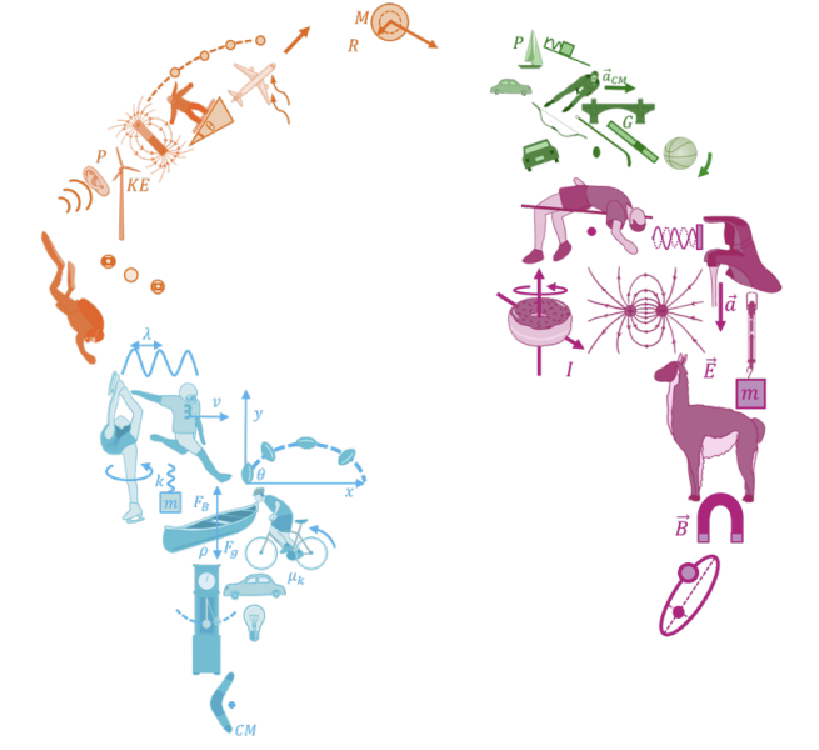
\includegraphics[width=4cm]{figures/BMDW/logo}
\end{textblock*}

\end{frame}

%%%%%%%%%%%%%%%%%%%%%%%%%%%%%%%%
%%Advertisements and such %%%%%%
%%%%%%%%%%%%%%%%%%%%%%%%%%%%%%%%

\twocolframe{Outline}
  {\tableofcontents[sections={1,2}, subsectionstyle=show/show]\thispagestyle{empty}}
  {\tableofcontents[sections={3}, subsectionstyle=show/show]}



%%%%%%%%%%%%%%%%%%%%%%%%%%%%%%%%%%%%%%%%%%%%%%%%%%%%%%%%%%%%%%
%% Annoucements                                         %%%%%%
%%%%%%%%%%%%%%%%%%%%%%%%%%%%%%%%%%%%%%%%%%%%%%%%%%%%%%%%%%%%%%

%%%%%%%%%%%%%%%%%%%%%%%%%%%%%%


\section{Pressure}
\label{sec:pressure}
\title{Pressure}


%%%%%%%%%%%%%%%%%%%%%%%%%
\begin{frame}
\titlepage
\thispagestyle{empty}
\end{frame}


%%%%%%%%%%%%%%%%%%%%%%%%%%%%%%%%%%%%%%%%%%%%%%%%%%%%%%%%%%%%%%%%%%%%%%%%%%%%%%%%%%%%%%%

\begin{frame}{Pressure}
\begin{itemize}
\item Defined as force per unit area:
\begin{align*}
P=\frac{F}{A}
\end{align*}
\item Scalar quantity.
\item Exerts a force that is normal to any surface.
\end{itemize}

\end{frame}


%%%%%%%%%%%%%%%%%%%%%%%%%%%%%%%%


%%%%%%%%%%%%%%%%%%%%%%%%%%%%%%%%
\subsection{Pressure in a fluid}
\label{subsec:pressureinafluid}
\twocolframesf{Pressure in a fluid}
{
\begin{itemize}
\item Pressure is a scalar, it does not have a direction.
\item A fluid (liquid or gas) cannot transmit force in a particular direction.
\item The pressure in a fluid is in all directions.
\item If there is a boundary on the fluid (e.g. a container), then the force from the pressure in the fluid is normal to the surface
\item You can think of the particles in the fluid as bouncing against the surfaces. The force required to change their momentum is the reaction force to the force associated with their pressure.
\end{itemize}
}
{

\begin{center}
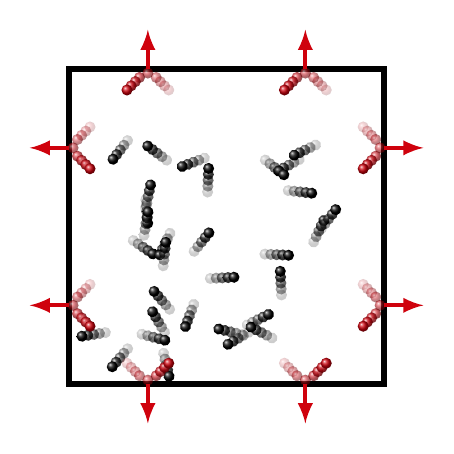
\begin{tikzpicture}[scale=1]
\tikzmath{
\L=4;
}
\scalebox{1}{

\draw[line width=2] (0,0) rectangle (\L,\L);

\foreach \i in {0,...,30}{
\tikzmath{
\xpos = 0.35*(1.3+rand)*\L;
\ypos = 0.35*(1.3+rand)*\L;
\th = 0.5*(1+rand)*360;
}
%\draw[color=black!50,line width=2pt] (\xpos,\ypos) -- +(\th:0.25);
\begin{scope}[shift={(\xpos,\ypos)}, rotate=\th]
\foreach \j in {1,...,5}{
\tikzmath{
 \xs=\j*0.075;
 \tra=\j*0.2;
}
\shade[ball color=black, opacity=\tra] (\xs,0)  circle (2pt);
}
\end{scope}
}

\coordinate (P1) at (0,3*\L/4);
\shade[ball color=myred, opacity=0.2] ($(P1)+(45:0.375)$) circle (2pt);
\shade[ball color=myred, opacity=0.3] ($(P1)+(45:0.30)$) circle (2pt);
\shade[ball color=myred, opacity=0.4] ($(P1)+(45:0.225)$) circle (2pt);
\shade[ball color=myred, opacity=0.5] ($(P1)+(45:0.15)$) circle (2pt);
\shade[ball color=myred, opacity=0.6] ($(P1)+(0.05,0)$) circle (2pt);
\shade[ball color=myred, opacity=0.7] ($(P1)+(-45:0.15)$) circle (2pt);
\shade[ball color=myred, opacity=0.8] ($(P1)+(-45:0.225)$) circle (2pt);
\shade[ball color=myred, opacity=0.9] ($(P1)+(-45:0.30)$) circle (2pt);
\shade[ball color=myred, opacity=1] ($(P1)+(-45:0.375)$) circle (2pt);
\draw[-latex, color=myred, line width=1.5] (P1) -- +(-0.5,0);

\coordinate (P1b) at (0,\L/4);
\shade[ball color=myred, opacity=0.2] ($(P1b)+(45:0.375)$) circle (2pt);
\shade[ball color=myred, opacity=0.3] ($(P1b)+(45:0.30)$) circle (2pt);
\shade[ball color=myred, opacity=0.4] ($(P1b)+(45:0.225)$) circle (2pt);
\shade[ball color=myred, opacity=0.5] ($(P1b)+(45:0.15)$) circle (2pt);
\shade[ball color=myred, opacity=0.6] ($(P1b)+(0.05,0)$) circle (2pt);
\shade[ball color=myred, opacity=0.7] ($(P1b)+(-45:0.15)$) circle (2pt);
\shade[ball color=myred, opacity=0.8] ($(P1b)+(-45:0.225)$) circle (2pt);
\shade[ball color=myred, opacity=0.9] ($(P1b)+(-45:0.30)$) circle (2pt);
\shade[ball color=myred, opacity=1] ($(P1b)+(-45:0.375)$) circle (2pt);
\draw[-latex, color=myred, line width=1.5] (P1b) -- +(-0.5,0);

\coordinate (P2) at (\L,\L/4);
\shade[ball color=myred, opacity=0.2] ($(P2)+(135:0.375)$) circle (2pt);
\shade[ball color=myred, opacity=0.3] ($(P2)+(135:0.30)$) circle (2pt);
\shade[ball color=myred, opacity=0.4] ($(P2)+(135:0.225)$) circle (2pt);
\shade[ball color=myred, opacity=0.5] ($(P2)+(135:0.15)$) circle (2pt);
\shade[ball color=myred, opacity=0.6] ($(P2)+(-0.05,0)$) circle (2pt);
\shade[ball color=myred, opacity=0.7] ($(P2)+(225:0.15)$) circle (2pt);
\shade[ball color=myred, opacity=0.8] ($(P2)+(225:0.225)$) circle (2pt);
\shade[ball color=myred, opacity=0.9] ($(P2)+(225:0.30)$) circle (2pt);
\shade[ball color=myred, opacity=1] ($(P2)+(225:0.375)$) circle (2pt);
\draw[-latex, color=myred, line width=1.5] (P2) -- +(0.5,0);

\coordinate (P2b) at (\L,3*\L/4);
\shade[ball color=myred, opacity=0.2] ($(P2b)+(135:0.375)$) circle (2pt);
\shade[ball color=myred, opacity=0.3] ($(P2b)+(135:0.30)$) circle (2pt);
\shade[ball color=myred, opacity=0.4] ($(P2b)+(135:0.225)$) circle (2pt);
\shade[ball color=myred, opacity=0.5] ($(P2b)+(135:0.15)$) circle (2pt);
\shade[ball color=myred, opacity=0.6] ($(P2b)+(-0.05,0)$) circle (2pt);
\shade[ball color=myred, opacity=0.7] ($(P2b)+(225:0.15)$) circle (2pt);
\shade[ball color=myred, opacity=0.8] ($(P2b)+(225:0.225)$) circle (2pt);
\shade[ball color=myred, opacity=0.9] ($(P2b)+(225:0.30)$) circle (2pt);
\shade[ball color=myred, opacity=1] ($(P2b)+(225:0.375)$) circle (2pt);
\draw[-latex, color=myred, line width=1.5] (P2b) -- +(0.5,0);

\coordinate (P3) at (3*\L/4,\L);
\shade[ball color=myred, opacity=0.2] ($(P3)+(-45:0.375)$) circle (2pt);
\shade[ball color=myred, opacity=0.3] ($(P3)+(-45:0.30)$) circle (2pt);
\shade[ball color=myred, opacity=0.4] ($(P3)+(-45:0.225)$) circle (2pt);
\shade[ball color=myred, opacity=0.5] ($(P3)+(-45:0.15)$) circle (2pt);
\shade[ball color=myred, opacity=0.6] ($(P3)+(0,-0.05)$) circle (2pt);
\shade[ball color=myred, opacity=0.7] ($(P3)+(225:0.15)$) circle (2pt);
\shade[ball color=myred, opacity=0.8] ($(P3)+(225:0.225)$) circle (2pt);
\shade[ball color=myred, opacity=0.9] ($(P3)+(225:0.30)$) circle (2pt);
\shade[ball color=myred, opacity=1] ($(P3)+(225:0.375)$) circle (2pt);
\draw[-latex, color=myred, line width=1.5] (P3) -- +(0,0.5);

\coordinate (P3b) at (\L/4,\L);
\shade[ball color=myred, opacity=0.2] ($(P3b)+(-45:0.375)$) circle (2pt);
\shade[ball color=myred, opacity=0.3] ($(P3b)+(-45:0.30)$) circle (2pt);
\shade[ball color=myred, opacity=0.4] ($(P3b)+(-45:0.225)$) circle (2pt);
\shade[ball color=myred, opacity=0.5] ($(P3b)+(-45:0.15)$) circle (2pt);
\shade[ball color=myred, opacity=0.6] ($(P3b)+(0,-0.05)$) circle (2pt);
\shade[ball color=myred, opacity=0.7] ($(P3b)+(225:0.15)$) circle (2pt);
\shade[ball color=myred, opacity=0.8] ($(P3b)+(225:0.225)$) circle (2pt);
\shade[ball color=myred, opacity=0.9] ($(P3b)+(225:0.30)$) circle (2pt);
\shade[ball color=myred, opacity=1] ($(P3b)+(225:0.375)$) circle (2pt);
\draw[-latex, color=myred, line width=1.5] (P3b) -- +(0,0.5);

\coordinate (P4) at (\L/4,0);
\shade[ball color=myred, opacity=0.2] ($(P4)+(135:0.375)$) circle (2pt);
\shade[ball color=myred, opacity=0.3] ($(P4)+(135:0.30)$) circle (2pt);
\shade[ball color=myred, opacity=0.4] ($(P4)+(135:0.225)$) circle (2pt);
\shade[ball color=myred, opacity=0.5] ($(P4)+(135:0.15)$) circle (2pt);
\shade[ball color=myred, opacity=0.6] ($(P4)+(0,0.05)$) circle (2pt);
\shade[ball color=myred, opacity=0.7] ($(P4)+(45:0.15)$) circle (2pt);
\shade[ball color=myred, opacity=0.8] ($(P4)+(45:0.225)$) circle (2pt);
\shade[ball color=myred, opacity=0.9] ($(P4)+(45:0.30)$) circle (2pt);
\shade[ball color=myred, opacity=1] ($(P4)+(45:0.375)$) circle (2pt);
\draw[-latex, color=myred, line width=1.5] (P4) -- +(0,-0.5);

\coordinate (P4b) at (3*\L/4,0);
\shade[ball color=myred, opacity=0.2] ($(P4b)+(135:0.375)$) circle (2pt);
\shade[ball color=myred, opacity=0.3] ($(P4b)+(135:0.30)$) circle (2pt);
\shade[ball color=myred, opacity=0.4] ($(P4b)+(135:0.225)$) circle (2pt);
\shade[ball color=myred, opacity=0.5] ($(P4b)+(135:0.15)$) circle (2pt);
\shade[ball color=myred, opacity=0.6] ($(P4b)+(0,0.05)$) circle (2pt);
\shade[ball color=myred, opacity=0.7] ($(P4b)+(45:0.15)$) circle (2pt);
\shade[ball color=myred, opacity=0.8] ($(P4b)+(45:0.225)$) circle (2pt);
\shade[ball color=myred, opacity=0.9] ($(P4b)+(45:0.30)$) circle (2pt);
\shade[ball color=myred, opacity=1] ($(P4b)+(45:0.375)$) circle (2pt);
\draw[-latex, color=myred, line width=1.5] (P4b) -- +(0,-0.5);
}

\end{tikzpicture}
\captionof*{figure}{\textit{Particles in the fluid bounce against the boundaries exerting an outward normal force.}}
\end{center}

}


%%%%%%%%%%%%%%%%%%%%%%%%%%%%%%%%



%%%%%%%%%%%%%%%%%%%%%%%%%%%%%%%%
\subsection{Equilibirem}
\label{subsec:equilibriem}
\twocolframesf{Hydrostatic equilibrium}
{
\begin{itemize}
\item Literally: Water not move equilibrium.
\item Think of an element of fluid that is not moving.
\end{itemize}
}
{
\begin{center}
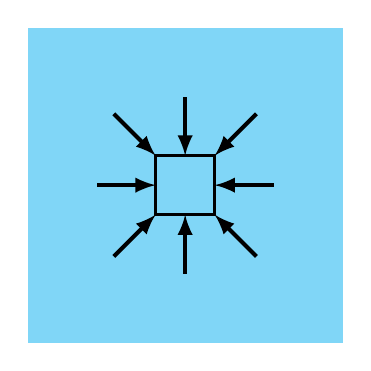
\begin{tikzpicture}[scale=1]
\tikzmath{
\L=4;
\abox=0.75;
}
\scalebox{1}{

\fill[color=cyan!50] (-\L/2,-\L/2) rectangle (\L/2,\L/2);
\draw[line width=1] (-\abox/2,-\abox/2) rectangle (\abox/2,\abox/2);

\draw[latex-, line width=1.5] (-\abox/2,-\abox/2) -- +(225:0.75);
\draw[latex-, line width=1.5] (\abox/2,-\abox/2) -- +(-45:0.75);
\draw[latex-, line width=1.5] (\abox/2,\abox/2) -- +(45:0.75);
\draw[latex-, line width=1.5] (-\abox/2,\abox/2) -- +(135:0.75);

\draw[latex-, line width=1.5] (0,\abox/2) -- +(90:0.75);
\draw[latex-, line width=1.5] (0,-\abox/2) -- +(-90:0.75);
\draw[latex-, line width=1.5] (\abox/2,0) -- +(0:0.75);
\draw[latex-, line width=1.5] (-\abox/2,0) -- +(180:0.75);
}

\end{tikzpicture}
\captionof*{figure}{\textit{A fluid element in hydrostatic equilibrium.}}
\end{center}
}


%%%%%%%%%%%%%%%%%%%%%%%%%%%%%%%%
\subsection{Pressure gradient}
\label{subsec:prssuregradient}
\twocolframesf{Pressure gradient in a fluid}
{
\begin{itemize}
\item In order for the fluid element to be in equilibrium, the net force on it must be zero:
\begin{align*}
\sum F_y=P_2A -mg- P_1A=0
\end{align*}
\item Using density for the mass:
\begin{align*}
m=\rho V = \rho A h
\end{align*}
\item Altogether:
\begin{align*}
P_2A -\rho A hg- P_1A&=0\\
P_2-P_1=\rho g h
\end{align*}

\end{itemize}
}
{
\vspace{-1.5cm}
\begin{center}
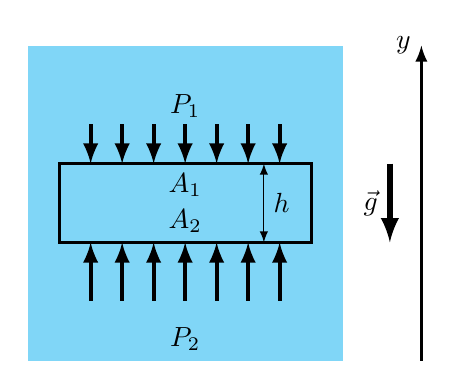
\begin{tikzpicture}[scale=1]
\tikzmath{
\L=4;
\abox=1;
}
\scalebox{1}{

\fill[color=cyan!50] (-\L/2,-\L/2) rectangle (\L/2,\L/2);

\draw[line width=1] (-0.4*\L,-\abox/2) rectangle (0.4*\L,\abox/2);


\foreach \xp in {-0.3,-0.2,-0.1,...,0.3}{
\draw[latex-,line width=1.5] (\xp*\L,\abox/2) -- +(0,0.5);
\draw[latex-,line width=1.5] (\xp*\L,-\abox/2) -- +(0,-0.75);
}

\draw[-latex, line width=1] (0.75*\L,-\L/2) -- +(0,\L) node[left]{$y$};
\draw[-latex, line width=2] (0.65*\L,\abox/2) -- +(0,-1) node[midway, left]{$\vec g$};

\draw[latex-latex] (0.25*\L,-\abox/2) --(0.25*\L, \abox/2) node[midway, right]{$h$};

\node[above] at (0,-\abox/2) {$A_2$};
\node[below] at (0,\abox/2) {$A_1$};


\node[above] at (0,-2*\abox) {$P_2$};
\node[below] at (0,1.5*\abox) {$P_1$};
}

\end{tikzpicture}
\captionof*{figure}{\textit{A fluid element in hydrostatic equilibrium, with gravity.}}
\end{center}

\only<2>{
In other words, the pressure increases as you move down:
\begin{align*}
P_2=P_1+\rho g h
\end{align*}
}
}


%%%%%%%%%%%%%%%%%%%%%%%%%%%%%%%%

\twocolframesf{If the fluid is \textit{compressible}}
{
\begin{itemize}
\item The density of the fluid can vary with pressure (e.g. if the fluid is a gas, like the Earth's atmosphere).
\item Then, we model an infinitesimal fluid element, small enough so that density is constant:
\begin{align*}
\frac{dP}{dy}&=-\rho g\\
\therefore P(y_2)-P(y_1)&= \int_{y_1}^{y_2} \rho(y) g dy
\end{align*}
\item For constant density, recover:
\begin{align*}
\int_{y_1}^{y_2} \rho(y) g dy = \rho g (y_2-y_1) = \rho g h
\end{align*}

\end{itemize}
}
{
\begin{center}
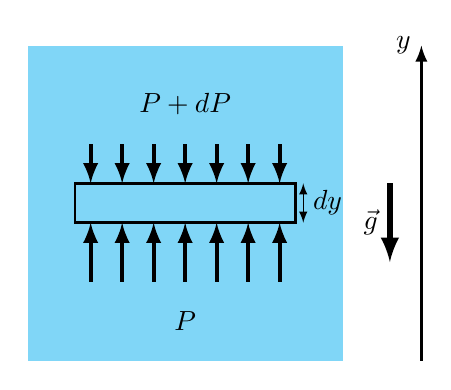
\begin{tikzpicture}[scale=1]
\tikzmath{
\L=4;
\abox=0.5;
}
\scalebox{1}{

\fill[color=cyan!50] (-\L/2,-\L/2) rectangle (\L/2,\L/2);

\draw[line width=1] (-0.35*\L,-\abox/2) rectangle (0.35*\L,\abox/2);


\foreach \xp in {-0.3,-0.2,-0.1,...,0.3}{
\draw[latex-,line width=1.5] (\xp*\L,\abox/2) -- +(0,0.5);
\draw[latex-,line width=1.5] (\xp*\L,-\abox/2) -- +(0,-0.75);
}

\draw[-latex, line width=1] (0.75*\L,-\L/2) -- +(0,\L) node[left]{$y$};
\draw[-latex, line width=2] (0.65*\L,\abox/2) -- +(0,-1) node[midway, left]{$\vec g$};

\draw[latex-latex] (0.375*\L,-\abox/2) --(0.375*\L, \abox/2) node[midway, right]{$dy$};

\node[above] at (0,1) {$P+dP$};
\node[below] at (0,-1.25) {$P$};
}

\end{tikzpicture}
\captionof*{figure}{\textit{A compressible fluid element in hydrostatic equilibrium. Note that $dP$ is negative in the figure.}}
\end{center}

}



%%%%%%%%%%%%%%%%%%%%%%%%%%%%%%%%
\subsection{Atmospheric pressure}
\begin{frame}{The Earth's atmosphere}
\begin{itemize}
\item A rough approximation is that density is proportional to pressure (e.g. ideal gas law).
\begin{align*}
\rho(y) = a P(y)
\end{align*}
where $a$ is just a constant of proportionality.

\item One finds that:
\begin{align*}
\frac{dP}{dy}&=-\rho g=-a P(y) g\\
\therefore P(y) &= P_0 e^{-agy}
\end{align*}

\item Pressure decreases exponentially with increasing altitude.
\end{itemize}
\end{frame}


%%%%%%%%%%%%%%%%%%%%%%%%%%%%%%%%
\subsection{Pascal's principle}
\label{subsec:pascalsprinciple}
\twocolframesf{Pascal’s principle}
{
\begin{itemize}
\item If you exert an external pressure on a fluid, the pressure in the fluid increases everywhere by the same amount.
\item<2-> The absolute pressure in, say, water, then depends on the atmospheric pressure, $P_0$:
\begin{align*}
P_2=P_0+P_1+\rho g h
\end{align*}
\item<2-> Or, in general, some distance $h$ below the surface:
\begin{align*}
P_2=P_0+\rho g h
\end{align*}
\end{itemize}
}
{
\only<1>{
\begin{center}
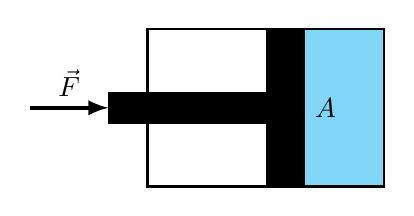
\begin{tikzpicture}[scale=1]
\tikzmath{
\abox=2;
}
\scalebox{1}{
\fill[color=cyan!50] (0,0) rectangle (\abox/2,\abox);
\draw[line width=1] (-\abox,0) rectangle (\abox/2,\abox);
\fill(-0.25*\abox,0) rectangle (0,\abox);
\fill(-1.25*\abox,0.4*\abox) rectangle (-0.25*\abox,0.6*\abox);
\draw[latex-, line width=1.5] (-1.25*\abox,0.5*\abox) -- +(-1,0) node[midway,above]{$\vec F$};
\node[right] at (0,\abox/2) {$A$};
}

\end{tikzpicture}
\captionof*{figure}{\textit{Pascal's principle: applying pressure externally to a fluid increases its pressure.}}
\end{center}
}

\only<2->{
\begin{center}
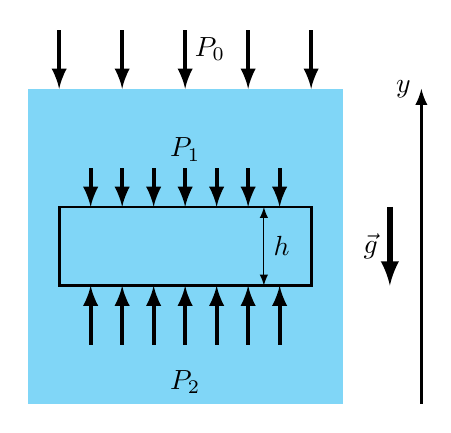
\begin{tikzpicture}[scale=1]
\tikzmath{
\L=4;
\abox=1;
}
\scalebox{1}{

\fill[color=cyan!50] (-\L/2,-\L/2) rectangle (\L/2,\L/2);

\draw[line width=1] (-0.4*\L,-\abox/2) rectangle (0.4*\L,\abox/2);

\foreach \xp in {-0.4,-0.2,0,...,0.4}{
\draw[latex-,line width=1.5] (\xp*\L,\L/2) -- +(0,0.75);
}
\node[right] at (0,2.5) {$P_0$};

\foreach \xp in {-0.3,-0.2,-0.1,...,0.3}{
\draw[latex-,line width=1.5] (\xp*\L,\abox/2) -- +(0,0.5);
\draw[latex-,line width=1.5] (\xp*\L,-\abox/2) -- +(0,-0.75);
}

\draw[-latex, line width=1] (0.75*\L,-\L/2) -- +(0,\L) node[left]{$y$};
\draw[-latex, line width=2] (0.65*\L,\abox/2) -- +(0,-1) node[midway, left]{$\vec g$};

\draw[latex-latex] (0.25*\L,-\abox/2) --(0.25*\L, \abox/2) node[midway, right]{$h$};

\node[above] at (0,-2*\abox) {$P_2$};
\node[below] at (0,1.5*\abox) {$P_1$};
}

\end{tikzpicture}
\captionof*{figure}{\textit{A fluid with atmospheric pressure on it.}}
\end{center}
}

}


%%%%%%%%%%%%%%%%%%%%%%%%%%%%%%%%



%%%%%%%%%%%%%%%%%%%%%%%%%%%%%%%%



%%%%%%%%%%%%%%%%%%%%%%%%%%%%%%%%



%%%%%%%%%%%%%%%%%%%%%%%%%%%%%%%%

\section{Hydrostatics/Dynamics}
\label{sec:hydrostaticsdynamics}
\title{Hydrostatics and Dynamics}


%%%%%%%%%%%%%%%%%%%%%%%%%
\begin{frame}
\titlepage
\thispagestyle{empty}
\end{frame}

%%%%%%%%%%%%%%%%%%%%%%%%%%%%%%%%



%%%%%%%%%%%%%%%%%%%%%%%%%%%%%%%%
\subsection{Buoyancy}
\label{subsec:buoyancy}
\twocolframe{Buoyancy}
{
\vspace{-0.25cm}
\begin{itemize}
\item Same effect as hydrostatic equilibrium.
\item There is a net upwards force on the fluid element because of the pressure gradient (due to gravity – pressure increases downwards).
\item If you replace the fluid element with an object, that pressure gradient and resulting upwards force does not go away!
\item Magnitude of the force is equal to the weight of the fluid displaced:
\begin{align*}
F_B=m_{fluid}g=\rho V g
\end{align*}
\item This does not change with depth!
\end{itemize}
}
{
\vspace{-0.75cm}
\begin{center}
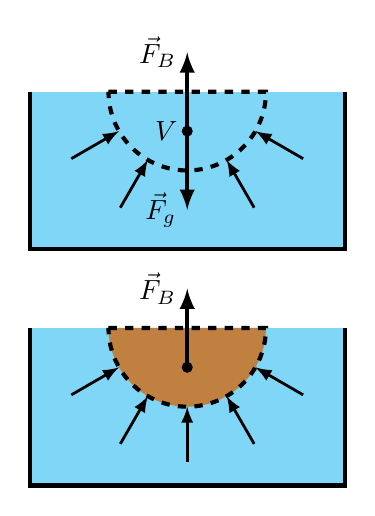
\begin{tikzpicture}[scale=1]
\tikzmath{
\L=4;
\R=1;
}
\scalebox{1}{

\fill[color=cyan!50] (-\L/2,-\L/2) rectangle (\L/2,0);
\draw[line width =1.5] (-\L/2,0) -- (-\L/2,-\L/2)  -- (\L/2,-\L/2) -- (\L/2,0);

\draw[line width=1.5, dashed] (-\R,0) -- (\R,0) arc(0:-180:\R);
\coordinate (P1) at (0,-\R/2);
\fill (P1) circle(2pt);
\draw[-latex, line width=1.5] (P1) -- +(0,1) node[left]{$\vec F_B$};
\draw[-latex, line width=1.5] (P1) -- +(0,-1) node[left]{$\vec F_g$};
\node[left] at  (0,-\R/2){$V$};

\foreach \th in {210,240,300, 330}{
 \draw[latex-,line width=1] (\th:\R) -- +(\th:0.7);
}

\begin{scope}[shift={(0,-0.75*\L)}]
\fill[color=cyan!50] (-\L/2,-\L/2) rectangle (\L/2,0);
\draw[line width =1.5] (-\L/2,0) -- (-\L/2,-\L/2)  -- (\L/2,-\L/2) -- (\L/2,0);

\draw[line width=1.5, dashed, fill=brown] (-\R,0) -- (\R,0) arc(0:-180:\R)--cycle;
\coordinate (P1) at (0,-\R/2);
\fill (P1) circle(2pt);
\draw[-latex, line width=1.5] (P1) -- +(0,1) node[left]{$\vec F_B$};


\foreach \th in {210,240,300,270,330}{
 \draw[latex-,line width=1] (\th:\R) -- +(\th:0.7);
}
\end{scope}

}

\end{tikzpicture}
\captionof*{figure}{\textit{A volume, $V$, supported by the same buoyancy force, regardless of being filled by fluid or an object.}}
\end{center}
}


%%%%%%%%%%%%%%%%%%%%%%%%%%%%%%%%



%%%%%%%%%%%%%%%%%%%%%%%%%%%%%%%%


%%%%%%%%%%%%%%%%%%%%%%%%%%%%%%%%
\subsection{Origin of buoyancy force}
\label{subsec:originofbuoyancyforce}
\twocolframesf{Buoyancy force comes from pressure gradient}
{
\begin{itemize}
\item At rest, there is a pressure gradient in the air that is downwards because of gravity.
\item When the car is accelerating, each element of the air must also accelerate with the car:
\begin{itemize}
\item The sum of the forces must be:
\begin{align*}
\sum F = ma =\rho V a
\end{align*}
\item The only way this can happen is if the pressure gradient is in a direction to accelerate the fluid with the car (must oppose gravity and go to the right).
\end{itemize}

\end{itemize}
}
{
\vspace{-0.5cm}
\begin{center}
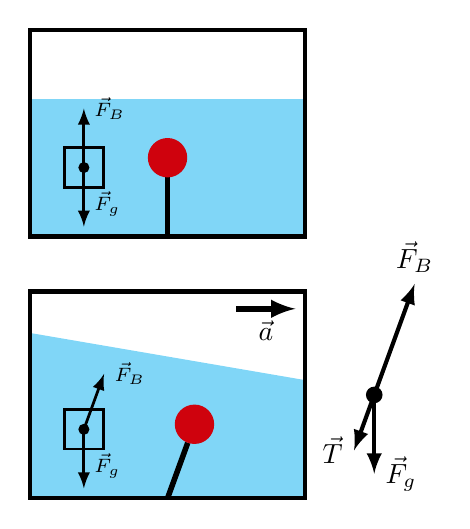
\begin{tikzpicture}[scale=1]
\tikzmath{
\L=3.5;
\abox=0.5;
}
\scalebox{1}{

\fill[color=cyan!50] (-\L/2,-\L/2) rectangle (\L/2,0);
\draw[line width =1.5] (-\L/2,\L/4) -- (-\L/2,-\L/2)  -- (\L/2,-\L/2) -- (\L/2,\L/4) --cycle;

\draw[line width =1] (-0.75*\L/2,-\L/4-\abox/2) rectangle +(\abox,\abox);
\coordinate (P) at ($ (-0.75*\L/2,-\L/4-\abox/2) +(\abox/2,\abox/2)$);
\fill (P) circle (2pt);
\draw[-latex, line width =1] (P) -- +(0,0.75) node[right]{\scriptsize $\vec F_B$};
\draw[-latex, line width =1] (P) -- +(0,-0.75) node[above right]{\scriptsize $\vec F_g$};

\draw[line width =2] (0,-\L/2) -- +(0,0.75);
\fill[color=myred] ($ (0, -\L/2)+(0,0.75)+(0,0.25) $) circle(0.25);

\begin{scope}[shift={(0,-0.95*\L)}]
\fill[color=cyan!50] (-\L/2,0.35) -- (-\L/2,-\L/2)  -- (\L/2,-\L/2) -- (\L/2,-0.25) --cycle;
\draw[line width =1.5] (-\L/2,\L/4) -- (-\L/2,-\L/2)  -- (\L/2,-\L/2) -- (\L/2,\L/4) --cycle;

\draw[line width =1] (-0.75*\L/2,-\L/4-\abox/2) rectangle +(\abox,\abox);
\coordinate (P) at ($ (-0.75*\L/2,-\L/4-\abox/2) +(\abox/2,\abox/2)$);
\fill (P) circle (2pt);
\draw[-latex, line width =1] (P) -- +(70:0.75) node[right]{\scriptsize $\vec F_B$};
\draw[-latex, line width =1] (P) -- +(0,-0.75) node[above right]{\scriptsize $\vec F_g$};

\draw[line width =2] (0,-\L/2) -- +(70:0.75);
\fill[color=myred] ($ (0, -\L/2)+(70:0.75)+(70:0.25) $) circle(0.25);

\draw[-latex,line width=2] (\L/4,0.75*\L/4) -- +(0.75,0) node[midway,below]{$\vec a$};

\coordinate (P) at (1.5*\L/2,-\L/8);
\fill (P) circle (3pt);
\draw[-latex, line width=1.5] (P) --+(0,-1) node[right]{$\vec F_g$};
\draw[-latex, line width=1.5] (P) --+(250:0.75) node[left]{$\vec T$};
\draw[-latex, line width=1.5] (P) --+(70:1.5) node[above]{$\vec F_B$};
\end{scope}


}

\end{tikzpicture}
\captionof*{figure}{\textit{A fluid accelerating in a container with a floating ballon. FBD of forces on balloon.}}
\end{center}
}


%%%%%%%%%%%%%%%%%%%%%%%%%%%%%%%%
\subsection{Hydrodynamics - flow rate}
\twocolframesf{Hydrodynamics - Flow rate, $Q$}
{
\begin{itemize}
\item Think of liquid moving through a horizontal pipe of cross section, $A$.
\item Continuity:
\begin{itemize}
\item What comes in must come out!
\item If we put in \SI{10}{l/min} into a pipe, then \SI{10}{l/min} must come out the other end (incompressible)
\end{itemize}
\item If the liquid flows at a speed, $v$, it covers a distance, $\Delta x$ in a time, $\Delta t$.  
\item The volume of fluid flowing per unit time is called the flow rate:
\begin{align*}
Q=\frac{\Delta V}{\Delta t}=\frac{\Delta x A}{\Delta t}=Av
\end{align*}
\end{itemize}
}
{
\begin{center}
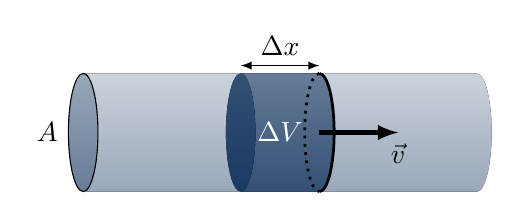
\begin{tikzpicture}[scale=1]
\tikzmath{
\L=5;
\R=0.75;
}
\scalebox{1}{

\fill[top color=myblue!20, bottom color=myblue!40] (0,\R) -- (\L,\R) arc (90:-90:\R/4 and \R) -- (0,-\R) arc(-90:90:\R/4 and \R);
\fill[top color=myblue!40, bottom color=myblue!60, draw=black]  (0,0) circle (\R/4 and \R);

\fill[top color=myblue!60, bottom color=myblue!80] (0.4*\L,\R) -- (0.6*\L,\R) arc (90:-90:\R/4 and \R) -- (0.4*\L,-\R) arc(-90:90:\R/4 and \R);
\fill[top color=myblue!80, bottom color=myblue!90]  (0.4*\L,0) circle (\R/4 and \R);
\draw[line width=1, dotted]  (0.6*\L,\R) arc (90:270:\R/4 and \R);
\draw[line width=1]  (0.6*\L,\R) arc (90:-90:\R/4 and \R);

\draw[-latex,line width=1.5]  (0.6*\L,0)--+(1,0) node[below]{$\vec v$};
\node[color=white] at (\L/2,0) {$\Delta V$};
\draw[latex-latex] (0.4*\L,\R+0.1) -- (0.6*\L,\R+0.1) node[midway,above]{$\Delta x$};
\node[left] at (-0.2,0) {$A$};
}

\end{tikzpicture}
\captionof*{figure}{\textit{A fluid element, of volume, $\Delta v$, moving in a pipe.}}
\end{center}
}


%%%%%%%%%%%%%%%%%%%%%%%%%%%%%%%%


%%%%%%%%%%%%%%%%%%%%%%%%%%%%%%%%
\subsection{Continuity}
\twocolframe{Continuity}
{
\begin{itemize}
\item What goes in must come out!
\item The flow rate in any point of the pipe must be the same:
\begin{align*}
Q_1 &=Q_2\\
A_1v_1 &= A_2 v_2\\
\therefore v_2 &= \frac{A_1}{A_2}v_1
\end{align*}
\end{itemize}
}
{
\begin{center}
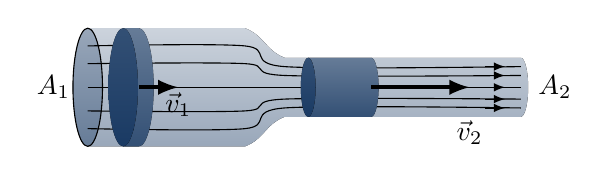
\begin{tikzpicture}[scale=1]
\tikzmath{
\L1=2;
\L2=3;
\R1=0.75;
\dh=0.5;
\R2=\R1/2;
\dx1=0.1*\L1;
\dx2=4*\dx1;
}
\scalebox{1}{

%The pipe:
\coordinate (P1) at (0,\R1) ;
\coordinate (P2) at (\L1,\R1);
\coordinate (P3) at (\L1+\dh,\R2);
\coordinate (P4) at (\L1+\dh+\L2,\R2);
\coordinate (P5) at ($(P4)-(0,2*\R2)$);
\coordinate (P6) at ($(P3)-(0,2*\R2)$);
\coordinate (P7) at ($(P2)-(0,2*\R1)$);
\coordinate (P8) at ($(P1)-(0,2*\R1)$);

\fill[top color=myblue!20, bottom color=myblue!40] (P1) -- (P2) ..controls ($(P2)+(0.25,-0.1)$) and ($(P3)+(-0.25,0.1)$) .. (P3) -- (P4) arc (90:-90:\R2/4 and \R2) -- (P6) ..controls ($(P6)+(-0.25,-0.1)$) and ($(P7)+(0.25,0.1)$) .. (P7) -- (P8) arc (-90:90:\R1/4 and \R1);
\fill[top color=myblue!40, bottom color=myblue!60, draw=black]  (0,0) circle (\R1/4 and \R1);
\draw plot [smooth] coordinates {($(P1)-(0,0.3*\R1)$) ($(P2)-(0,0.3*\R1)$)  ($(P3)-(0,0.3*\R2)$)  ($(P4)-(0,0.3*\R2)$) } ;
\draw plot [smooth] coordinates {($(P1)-(0,0.6*\R1)$) ($(P2)-(0,0.6*\R1)$)  ($(P3)-(0,0.6*\R2)$)  ($(P4)-(0,0.6*\R2)$) } ;
\draw ($(P1)-(0,\R1)$) -- ($(P4)-(0,\R2)$) ;
\draw plot [smooth] coordinates {($(P8)+(0,0.3*\R1)$) ($(P7)+(0,0.3*\R1)$)  ($(P6)+(0,0.3*\R2)$)  ($(P5)+(0,0.3*\R2)$) } ;
\draw plot [smooth] coordinates {($(P8)+(0,0.6*\R1)$) ($(P7)+(0,0.6*\R1)$)  ($(P6)+(0,0.6*\R2)$)  ($(P5)+(0,0.6*\R2)$) } ;
\draw[-latex] (\L1+\dh+0.85*\L2,0.7*\R2) -- +(0.25,0);
\draw[-latex] (\L1+\dh+0.85*\L2,0.4*\R2) -- +(0.25,0);
\draw[-latex] (\L1+\dh+0.85*\L2,0) -- +(0.25,0);
\draw[-latex] (\L1+\dh+0.85*\L2,-0.7*\R2) -- +(0.25,0);
\draw[-latex] (\L1+\dh+0.85*\L2,-0.4*\R2) -- +(0.25,0);

\fill[top color=myblue!60, bottom color=myblue!80] (0.225*\L1,\R1) -- (0.225*\L1+\dx1,\R1) arc (90:-90:\R1/4 and \R1) -- (0.225*\L1,-\R1) arc(-90:90:\R1/4 and \R1);
\fill[top color=myblue!80, bottom color=myblue!90]  (0.225*\L1,0) circle (\R1/4 and \R1);
\draw[-latex,line width=1.5]  (0.225*\L1+\dx1,0)--+(0.5,0) node[below=-2pt]{$\vec v_1$};

\fill[top color=myblue!60, bottom color=myblue!80] (\L1+\dh+0.1*\L2,\R2) -- (\L1+\dh+0.1*\L2+\dx2,\R2) arc (90:-90:\R2/4 and \R2) -- (\L1+\dh+0.1*\L2,-\R2) arc(-90:90:\R2/4 and \R2);
\fill[top color=myblue!80, bottom color=myblue!90]  (\L1+\dh+0.1*\L2,0) circle (\R2/4 and \R2);
\draw[-latex,line width=1.5]  (\L1+\dh+0.1*\L2+\dx2,0) -- +(1.25,0) node[below=8pt]{$\vec v_2$};

\node[left] at (-0.1,0) {$A_1$};
\node[right] at (\L1+\L2+\dh+0.1,0) {$A_2$};
}

\end{tikzpicture}
\captionof*{figure}{\textit{A fluid element moving in a pipe that gets narrower, laminar flow.}}
\end{center}
}


%%%%%%%%%%%%%%%%%%%%%%%%%%%%%%%%







\section{Bernoulli's Principle}
\label{sec:bernoullisprinciple}
\title{Bernoulli's Principle}


%%%%%%%%%%%%%%%%%%%%%%%%%
\begin{frame}
\titlepage
\thispagestyle{empty}
\end{frame}


%%%%%%%%%%%%%%%%%%%%%%%%%%%%%%%%



\subsection{Definition and derivation}
\label{subsec:definitionandderivation}
\twocolframe{Bernoulli's Principle}
{
\only<1,2>{
\begin{itemize}
\item Describes the laminar flow of an incompressible fluid with no friction (no viscosity).
\item Model the motion of a fluid element as it moves through a pipe that changes height and cross-section (most general case).
\end{itemize}
}
\only<3>{
\begin{itemize}
\item Apply Work-Energy Theorem to the fluid element.
\item The force from the pressure at the bottom does positive work on the fluid element:
\begin{align*}
W_1=F_1\Delta x = (P_1A_1)(v_1\Delta t)
\end{align*}
\item The force from the pressure at the top does negative work on the fluid element:
\begin{align*}
W_2=-F_2\Delta x = -(P_2A_2)(v_2\Delta t)
\end{align*}
\end{itemize}
}
\only<4>{
\begin{itemize}
\item Gravity does negative work:
\begin{align*}
W_g=-\Delta m g (y_2-y_1)
\end{align*}
where the fluid element has mass:
\begin{align*}
\Delta m = \rho V=\rho A_1 v_1 \Delta t = \rho A_2 v_2 \Delta t
\end{align*}
\item The total work done on the fluid element must equal the change in kinetic energy:
\begin{align*}
W_1+W_2+W_g=\Delta K =\frac{1}{2} \Delta m (v_2^2-v_1^2)
\end{align*}
\end{itemize}
}
\only<5>{
\begin{itemize}
\item All together (note $A_1v_1\Delta t = A_2 v_2 \Delta t$):
\begin{align*}
&(P_1A_1)(v_1\Delta t) - (P_2A_2)(v_2\Delta t) \\
&-\rho A_1 v_1 \Delta t  g (y_2-y_1) = \frac{1}{2} \rho A_1 v_1 \Delta t  (v_2^2-v_1^2)\\
&\therefore P_1+\frac{1}{2}\rho v_1^2+\rho g y_1= P_2+\frac{1}{2}\rho v_2^2+\rho g y_2
\end{align*}

\item This looks a lot like conservation of mechanical energy (\textit{it is!}):
\begin{align*}
E=K_1+U_2=K_2+U_2=\text{const.}\\
\Aboxed{E = P+\frac{1}{2}\rho v^2+\rho g y =\text{const.}}
\end{align*}
\end{itemize}
}
\only<6>{
\begin{align*}
\Aboxed{E = P+\frac{1}{2}\rho v^2+\rho g y =\text{const.}}
\end{align*}
\begin{itemize}
\item Think of $\frac{1}{2}\rho v^2$ as the kinetic energy of the fluid (energy per volume).
\item Think of $\rho g y$ as grav potential energy (per volume).
\item Think of $P$ as an additional potential energy (it's really the work being done by pressure, per unit volume).
\end{itemize}
}

}
{
\begin{center}
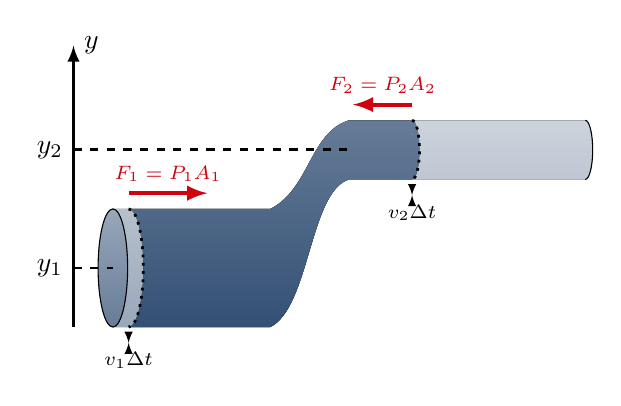
\begin{tikzpicture}[scale=1]
\tikzmath{
\L1=2;%first section
\dh=1;%transition length
\h=1.5;%transution height
\L2=3;%second section
\R1=0.75;%first section
\R2=\R1/2;%second section
\dx1=0.1*\L1;
\dx2=\dx1;
}
\scalebox{1}{
\only<2-6>{
\tikzmath{
\dx2=0.3*\L1;
}
}

%The pipe:
\coordinate (P1) at (0,\R1) ;
\coordinate (P2) at (\L1,\R1);
\coordinate (P3) at (\L1+\dh,\R2+\h);
\coordinate (P4) at (\L1+\dh+\L2,\R2+\h);
\coordinate (P5) at ($(P4)-(0,2*\R2)$);
\coordinate (P6) at ($(P3)-(0,2*\R2)$);
\coordinate (P7) at ($(P2)-(0,2*\R1)$);
\coordinate (P8) at ($(P1)-(0,2*\R1)$);

\fill[top color=myblue!20, bottom color=myblue!40] (P1) -- (P2) ..controls ($(P2)+(0.5,0.25)$) and ($(P3)-(0.5,0.15)$) .. (P3) -- (P4) arc (90:-90:\R2/4 and \R2) -- (P6) ..controls ($(P6)-(0.5,0.15)$) and ($(P7)+(0.5,0.25)$) .. (P7) -- (P8) arc (-90:90:\R1/4 and \R1);
\fill[top color=myblue!40, bottom color=myblue!60, draw=black]  (0,0) circle (\R1/4 and \R1);
\draw (P4) arc (90:-90:\R2/4 and \R2);

%The fluid element
\coordinate (F1) at (\dx2,\R1) ;
\coordinate (F2) at (\L1,\R1);
\coordinate (F3) at (\L1+\dh,\R2+\h);
\coordinate (F4) at (\L1+\dh+4*\dx2,\R2+\h);
\coordinate (F5) at ($(F4)-(0,2*\R2)$);
\coordinate (F6) at ($(F3)-(0,2*\R2)$);
\coordinate (F7) at ($(F2)-(0,2*\R1)$);
\coordinate (F8) at ($(F1)-(0,2*\R1)$);

\fill[top color=myblue!60, bottom color=myblue!80] (F1) -- (F2) ..controls ($(P2)+(0.5,0.25)$) and ($(P3)-(0.5,0.15)$) .. (F3) -- (F4) arc (90:-90:\R2/4 and \R2) -- (F6) ..controls ($(P6)-(0.5,0.15)$) and ($(P7)+(0.5,0.25)$) .. (F7) -- (F8) arc (-90:90:\R1/4 and \R1);

%coordinate system
\draw[-latex, line width=1] (-0.5,-\R1) -- +(0,\h+2*\R1+\R2+0.2) node[right] {$y$};
\draw[dashed, line width=1] (-0.5,0) node[left]{$y_1$} -- (0,0);
\draw[dashed, line width=1] (-0.5,\h) node[left]{$y_2$} -- (\L1+\dh,\h);
%Forces
\draw[-latex, line width=1.5,color=myred] (\dx2,\R1+0.2) -- +(1,0) node[midway,above]{\scriptsize $F_1=P_1A_1$};
\draw[-latex, line width=1.5,color=myred] (\L1+\dh+4*\dx2,\h+\R2+0.2) -- +(-0.75,0) node[midway,above]{\scriptsize $F_2=P_2A_2$};

\only<2-6>{
\draw[line width=1, dotted] (\dx1,\R1) arc(90:-90:\R1/4 and \R1);
\draw[line width=1, dotted]  (\L1+\dh+4*\dx1,\R2+\h) arc (90:-90:\R2/4 and \R2);
\draw[latex-latex] (\dx1,-\R1-0.2) -- (\dx2,-\R1-0.2) node[midway,below]{\scriptsize $v_1\Delta t$};
\draw[latex-latex] (\L1+\dh+4*\dx1,\h-\R2-0.2) -- (\L1+\dh+4*\dx2,\h-\R2-0.2) node[midway,below]{\scriptsize $v_2\Delta t$};
}
}

\end{tikzpicture}
\captionof*{figure}{\textit{A fluid element moving in a pipe that gets narrower while changing height. The motion is driven by a change in pressure (from high to low).\only<2>{ After a time $\Delta t$}}}
\end{center}
}


%%%%%%%%%%%%%%%%%%%%%%%%%%%%%%%%



%%%%%%%%%%%%%%%%%%%%%%%%%%%%%%%%



%%%%%%%%%%%%%%%%%%%%%%%%%%%%%%%%

\twocolframe{Recall: Flow rate and continuity}
{
\begin{itemize}
\item Define (volume) flow rate, $Q$:
\begin{align*}
Q=\frac{\Delta V}{\Delta t}=\frac{\Delta x A}{\Delta t}=Av
\end{align*}
\item Continuity:
\begin{itemize}
\item What comes in must come out (incompressible):
\begin{align*}
\therefore A_1 v_1 &= A_2 v_2
\end{align*}
\item For \textit{compressible} fluid, use the mass instead of the volume:
\begin{align*}
\frac{\Delta m}{\Delta t}&=\rho \frac{\Delta V}{\Delta t}=\rho Av\\
\therefore \rho_1 A_1 v_1 &=\rho_2 A_2 v_2
\end{align*}
\end{itemize}

\end{itemize}
}
{
\begin{center}
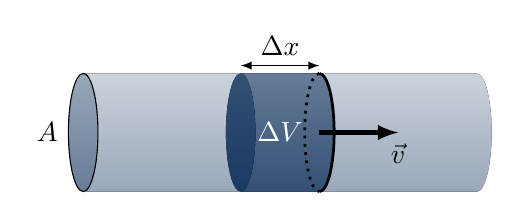
\begin{tikzpicture}[scale=1]
\tikzmath{
\L=5;
\R=0.75;
}
\scalebox{1}{

\fill[top color=myblue!20, bottom color=myblue!40] (0,\R) -- (\L,\R) arc (90:-90:\R/4 and \R) -- (0,-\R) arc(-90:90:\R/4 and \R);
\fill[top color=myblue!40, bottom color=myblue!60, draw=black]  (0,0) circle (\R/4 and \R);

\fill[top color=myblue!60, bottom color=myblue!80] (0.4*\L,\R) -- (0.6*\L,\R) arc (90:-90:\R/4 and \R) -- (0.4*\L,-\R) arc(-90:90:\R/4 and \R);
\fill[top color=myblue!80, bottom color=myblue!90]  (0.4*\L,0) circle (\R/4 and \R);
\draw[line width=1, dotted]  (0.6*\L,\R) arc (90:270:\R/4 and \R);
\draw[line width=1]  (0.6*\L,\R) arc (90:-90:\R/4 and \R);

\draw[-latex,line width=1.5]  (0.6*\L,0)--+(1,0) node[below]{$\vec v$};
\node[color=white] at (\L/2,0) {$\Delta V$};
\draw[latex-latex] (0.4*\L,\R+0.1) -- (0.6*\L,\R+0.1) node[midway,above]{$\Delta x$};
\node[left] at (-0.2,0) {$A$};
}

\end{tikzpicture}
\captionof*{figure}{\textit{A fluid element, of volume, $\Delta v$, moving in a pipe.}}
\end{center}

\begin{center}
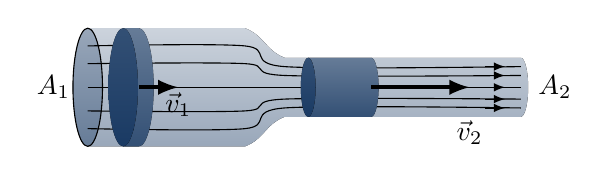
\begin{tikzpicture}[scale=1]
\tikzmath{
\L1=2;
\L2=3;
\R1=0.75;
\dh=0.5;
\R2=\R1/2;
\dx1=0.1*\L1;
\dx2=4*\dx1;
}
\scalebox{1}{

%The pipe:
\coordinate (P1) at (0,\R1) ;
\coordinate (P2) at (\L1,\R1);
\coordinate (P3) at (\L1+\dh,\R2);
\coordinate (P4) at (\L1+\dh+\L2,\R2);
\coordinate (P5) at ($(P4)-(0,2*\R2)$);
\coordinate (P6) at ($(P3)-(0,2*\R2)$);
\coordinate (P7) at ($(P2)-(0,2*\R1)$);
\coordinate (P8) at ($(P1)-(0,2*\R1)$);

\fill[top color=myblue!20, bottom color=myblue!40] (P1) -- (P2) ..controls ($(P2)+(0.25,-0.1)$) and ($(P3)+(-0.25,0.1)$) .. (P3) -- (P4) arc (90:-90:\R2/4 and \R2) -- (P6) ..controls ($(P6)+(-0.25,-0.1)$) and ($(P7)+(0.25,0.1)$) .. (P7) -- (P8) arc (-90:90:\R1/4 and \R1);
\fill[top color=myblue!40, bottom color=myblue!60, draw=black]  (0,0) circle (\R1/4 and \R1);
\draw plot [smooth] coordinates {($(P1)-(0,0.3*\R1)$) ($(P2)-(0,0.3*\R1)$)  ($(P3)-(0,0.3*\R2)$)  ($(P4)-(0,0.3*\R2)$) } ;
\draw plot [smooth] coordinates {($(P1)-(0,0.6*\R1)$) ($(P2)-(0,0.6*\R1)$)  ($(P3)-(0,0.6*\R2)$)  ($(P4)-(0,0.6*\R2)$) } ;
\draw ($(P1)-(0,\R1)$) -- ($(P4)-(0,\R2)$) ;
\draw plot [smooth] coordinates {($(P8)+(0,0.3*\R1)$) ($(P7)+(0,0.3*\R1)$)  ($(P6)+(0,0.3*\R2)$)  ($(P5)+(0,0.3*\R2)$) } ;
\draw plot [smooth] coordinates {($(P8)+(0,0.6*\R1)$) ($(P7)+(0,0.6*\R1)$)  ($(P6)+(0,0.6*\R2)$)  ($(P5)+(0,0.6*\R2)$) } ;
\draw[-latex] (\L1+\dh+0.85*\L2,0.7*\R2) -- +(0.25,0);
\draw[-latex] (\L1+\dh+0.85*\L2,0.4*\R2) -- +(0.25,0);
\draw[-latex] (\L1+\dh+0.85*\L2,0) -- +(0.25,0);
\draw[-latex] (\L1+\dh+0.85*\L2,-0.7*\R2) -- +(0.25,0);
\draw[-latex] (\L1+\dh+0.85*\L2,-0.4*\R2) -- +(0.25,0);

\fill[top color=myblue!60, bottom color=myblue!80] (0.225*\L1,\R1) -- (0.225*\L1+\dx1,\R1) arc (90:-90:\R1/4 and \R1) -- (0.225*\L1,-\R1) arc(-90:90:\R1/4 and \R1);
\fill[top color=myblue!80, bottom color=myblue!90]  (0.225*\L1,0) circle (\R1/4 and \R1);
\draw[-latex,line width=1.5]  (0.225*\L1+\dx1,0)--+(0.5,0) node[below=-2pt]{$\vec v_1$};

\fill[top color=myblue!60, bottom color=myblue!80] (\L1+\dh+0.1*\L2,\R2) -- (\L1+\dh+0.1*\L2+\dx2,\R2) arc (90:-90:\R2/4 and \R2) -- (\L1+\dh+0.1*\L2,-\R2) arc(-90:90:\R2/4 and \R2);
\fill[top color=myblue!80, bottom color=myblue!90]  (\L1+\dh+0.1*\L2,0) circle (\R2/4 and \R2);
\draw[-latex,line width=1.5]  (\L1+\dh+0.1*\L2+\dx2,0) -- +(1.25,0) node[below=8pt]{$\vec v_2$};

\node[left] at (-0.1,0) {$A_1$};
\node[right] at (\L1+\L2+\dh+0.1,0) {$A_2$};
}

\end{tikzpicture}
\captionof*{figure}{\textit{A fluid element moving in a pipe that gets narrower, laminar flow.}}
\end{center}

}


%%%%%%%%%%%%%%%%%%%%%%%%%%%%%%%%
\twocolframe{Bernoulli's Principle}
{
\only<1>{
\begin{itemize}
\item Describes the laminar flow of an incompressible fluid with no friction (no viscosity).
\item Model the motion of a fluid element as it moves through a pipe that changes height and cross-section (most general case).
\end{itemize}
}
\only<2>{
\begin{align*}
\Aboxed{E = P+\frac{1}{2}\rho v^2+\rho g y =\text{const.}}
\end{align*}
\begin{itemize}
\item Think of $\frac{1}{2}\rho v^2$ as the kinetic energy of the fluid (energy per volume).
\item Think of $\rho g y$ as gravitational potential energy (per volume).
\item Think of $P$ as an additional potential energy (per unit volume) due to the pressure in the fluid. It wants to flow where that energy (pressure) is lower.
\end{itemize}
}

}
{
\begin{center}
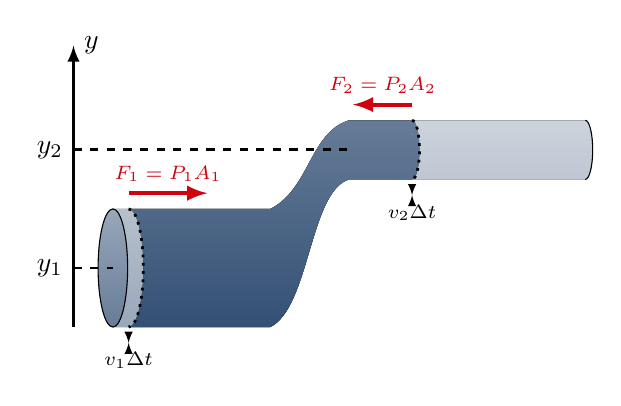
\begin{tikzpicture}[scale=1]
\tikzmath{
\L1=2;%first section
\dh=1;%transition length
\h=1.5;%transution height
\L2=3;%second section
\R1=0.75;%first section
\R2=\R1/2;%second section
\dx1=0.1*\L1;
\dx2=\dx1;
}
\scalebox{1}{
\only<2>{
\tikzmath{
\dx2=0.3*\L1;
}
}

%The pipe:
\coordinate (P1) at (0,\R1) ;
\coordinate (P2) at (\L1,\R1);
\coordinate (P3) at (\L1+\dh,\R2+\h);
\coordinate (P4) at (\L1+\dh+\L2,\R2+\h);
\coordinate (P5) at ($(P4)-(0,2*\R2)$);
\coordinate (P6) at ($(P3)-(0,2*\R2)$);
\coordinate (P7) at ($(P2)-(0,2*\R1)$);
\coordinate (P8) at ($(P1)-(0,2*\R1)$);

\fill[top color=myblue!20, bottom color=myblue!40] (P1) -- (P2) ..controls ($(P2)+(0.5,0.25)$) and ($(P3)-(0.5,0.15)$) .. (P3) -- (P4) arc (90:-90:\R2/4 and \R2) -- (P6) ..controls ($(P6)-(0.5,0.15)$) and ($(P7)+(0.5,0.25)$) .. (P7) -- (P8) arc (-90:90:\R1/4 and \R1);
\fill[top color=myblue!40, bottom color=myblue!60, draw=black]  (0,0) circle (\R1/4 and \R1);
\draw (P4) arc (90:-90:\R2/4 and \R2);

%The fluid element
\coordinate (F1) at (\dx2,\R1) ;
\coordinate (F2) at (\L1,\R1);
\coordinate (F3) at (\L1+\dh,\R2+\h);
\coordinate (F4) at (\L1+\dh+4*\dx2,\R2+\h);
\coordinate (F5) at ($(F4)-(0,2*\R2)$);
\coordinate (F6) at ($(F3)-(0,2*\R2)$);
\coordinate (F7) at ($(F2)-(0,2*\R1)$);
\coordinate (F8) at ($(F1)-(0,2*\R1)$);

\fill[top color=myblue!60, bottom color=myblue!80] (F1) -- (F2) ..controls ($(P2)+(0.5,0.25)$) and ($(P3)-(0.5,0.15)$) .. (F3) -- (F4) arc (90:-90:\R2/4 and \R2) -- (F6) ..controls ($(P6)-(0.5,0.15)$) and ($(P7)+(0.5,0.25)$) .. (F7) -- (F8) arc (-90:90:\R1/4 and \R1);

%coordinate system
\draw[-latex, line width=1] (-0.5,-\R1) -- +(0,\h+2*\R1+\R2+0.2) node[right] {$y$};
\draw[dashed, line width=1] (-0.5,0) node[left]{$y_1$} -- (0,0);
\draw[dashed, line width=1] (-0.5,\h) node[left]{$y_2$} -- (\L1+\dh,\h);
%Forces
\draw[-latex, line width=1.5,color=myred] (\dx2,\R1+0.2) -- +(1,0) node[midway,above]{\scriptsize $F_1=P_1A_1$};
\draw[-latex, line width=1.5,color=myred] (\L1+\dh+4*\dx2,\h+\R2+0.2) -- +(-0.75,0) node[midway,above]{\scriptsize $F_2=P_2A_2$};

\only<2>{
\draw[line width=1, dotted] (\dx1,\R1) arc(90:-90:\R1/4 and \R1);
\draw[line width=1, dotted]  (\L1+\dh+4*\dx1,\R2+\h) arc (90:-90:\R2/4 and \R2);
\draw[latex-latex] (\dx1,-\R1-0.2) -- (\dx2,-\R1-0.2) node[midway,below]{\scriptsize $v_1\Delta t$};
\draw[latex-latex] (\L1+\dh+4*\dx1,\h-\R2-0.2) -- (\L1+\dh+4*\dx2,\h-\R2-0.2) node[midway,below]{\scriptsize $v_2\Delta t$};
}
}

\end{tikzpicture}
\captionof*{figure}{\textit{A fluid element moving in a pipe that gets narrower while changing height.\only<2>{ After a time $\Delta t$}}}
\end{center}
}




%%%%%%%%%%%%%%%%%%%%%%%%%%%%%%%%




%%%%%%%%%%%%%%%%%%%%%%%%%%%%%%%%
\subsection{Example: strong winds}
\label{subsec:examplestrongwinds}
\twocolframesf{Example: Strong Winds}
{
\begin{itemize}
\item This is how strong winds blow roods off your house!
\end{itemize}
\capfig{0.7}{figures/FluidMechanics/roof1}{}
}
{
\vspace{2cm}
\capfig{1}{figures/FluidMechanics/roof2}{}

}


%%%%%%%%%%%%%%%%%%%%%%%%%%%%%%%%


%%%%%%%%%%%%%%%%%%%%%%%%%%%%%%%%

%%%%%%%%%%%%%%%%%%%%%%%%%%%%%%%%
\subsection{Viscosity}
\label{subsec:viscocity}
\twocolframesf{Viscosity}
{
\begin{itemize}
\item In reality, fluids have ``viscosity''. Think of maple syrup as being more viscous than water.
\item Viscosity is the results of internal friction of the fluid molecules with each other.
\item We can define it based on imagining a stationary fluid between 2 plates and measuring the force required to pull the top plate at constant speed $v$:
\begin{align*}
F\propto \frac{Av}{l} \;\;\rightarrow\;\; F=\eta \frac{Av}{l}
\end{align*}
\item A pressure difference is required to push fluid through a pipe, since the fluid ``sticks'' to the walls. Think: ``syringe full of maple syrup''.
\end{itemize}
}
{
\begin{center}
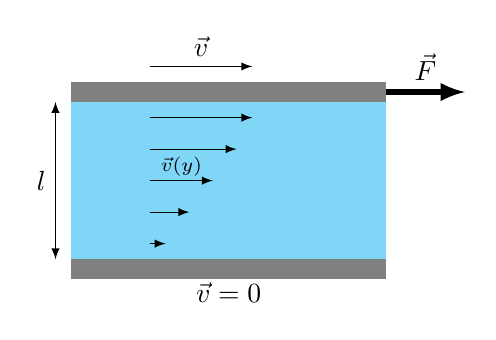
\begin{tikzpicture}[scale=1]
\tikzmath{
\L=4;
\h=2;
\dy=0.25;
}
\scalebox{1}{


\fill[color=cyan!50] (-\L/2,0) rectangle (\L/2,\h);
\fill[color=black!50] (-\L/2,\h) rectangle (\L/2,\h+\dy);
\fill[color=black!50] (-\L/2,0) rectangle (\L/2,-\dy);

\draw[latex-latex] (-\L/2-0.2,0) -- +(0,\L/2) node[midway, left]{$l$};

\draw[-latex, line width=2]  (\L/2,\h+0.5*\dy) -- +(1,0) node[midway,above] {$\vec F$};
\node[below=5pt] (0,-\dy) {$\vec v=0$};
\draw[-latex] (-\L/4,\h+\dy+0.2) -- +(1.3,0) node[midway,above] {$\vec v$};

\draw[-latex] (-\L/4,0.9*\h) -- +(1.3,0) ;
\draw[-latex] (-\L/4,0.7*\h) -- +(1.1,0) ;
\draw[-latex] (-\L/4,0.5*\h) -- +(0.8,0) node[midway,above=-2pt] {\scriptsize $\vec v(y)$} ;
\draw[-latex] (-\L/4,0.3*\h) -- +(0.5,0) ;
\draw[-latex] (-\L/4,0.1*\h) -- +(0.2,0) ;
}

\end{tikzpicture}
\captionof*{figure}{\textit{Fluid between two plates. The bottom plate is stationary and the one on top is pulled with a force, $\vec F$, at a constant speed, $v$. Different layers in the fluid move at different speeds.}}
\end{center}
}


%%%%%%%%%%%%%%%%%%%%%%%%%%%%%%%%
\subsection{Poiseuille flow}
\label{subsec:poiseuilleflow}
\twocolframesf{Poiseuille flow}
{
\begin{itemize}
\item The flow rate is proportional to the pressure difference across the pipe:
\begin{align*}
Q\propto \Delta P
\end{align*}
\item The constant of proportionality is called the resistance of the pipe (one over $R$, actually):
\begin{align*}
Q= \frac{1}{R} \Delta P
\end{align*}
\item We can write this as:
\begin{align*}
\Delta P = QR
\end{align*}
\item For a horizontal pipe: $R= \frac{8\eta L}{\pi r^4}$

\end{itemize}
}
{
\vspace{-1cm}
\begin{center}
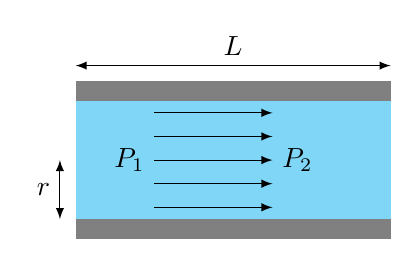
\begin{tikzpicture}[scale=1]
\tikzmath{
\L=4;
\h=1.5;
\dy=0.25;
}
\scalebox{1}{

\fill[color=cyan!50] (-\L/2,0) rectangle (\L/2,\h);
\fill[color=black!50] (-\L/2,\h) rectangle (\L/2,\h+\dy);
\fill[color=black!50] (-\L/2,0) rectangle (\L/2,-\dy);

\draw[-latex] (-\L/4,0.9*\h) -- +(1.5,0) ;
\draw[-latex] (-\L/4,0.7*\h) -- +(1.5,0) ;
\draw[-latex] (-\L/4,0.5*\h) node[left]{$P_1$}  -- +(1.5,0) node[right]{$P_2$};
\draw[-latex] (-\L/4,0.3*\h) -- +(1.5,0) ;
\draw[-latex] (-\L/4,0.1*\h) -- +(1.5,0) ;

\draw[latex-latex] (-\L/2,\h+\dy+0.2) -- +(\L,0) node[midway,above]{$L$};
\draw[latex-latex] (-\L/2-0.2,0) -- +(0,\h/2) node[midway,left]{$r$};

}

\end{tikzpicture}
\captionof*{figure}{\textit{Poiseuille flow in a pipe due to a pressure difference.}}
\end{center}
\begin{block}{Consequences}
\begin{itemize}
\item If there is no flow through the pipe, then there is no drop in pressure along the pipe.
\item If there is flow through the pipe, the pressure must drop along the pipe.
\end{itemize}
\end{block}


}


%%%%%%%%%%%%%%%%%%%%%%%%%%%%%%%%


%%%%%%%%%%%%%%%%%%%%%%%%%%%%%%%%


%%%%%%%%%%%%%%%%%%%%%%%%%%%%%%%%
\tikzset{%
  raindrop/.pic={
    code={\tikzset{scale=1/10}
 \clip [preaction={color=cyan!50}]
 (0,0)  .. controls ++(0,-1) and ++(0,1) .. (1,-2)
 arc (360:180:1)
 .. controls ++(0,1) and ++(0,-1) .. (0,0) -- cycle;
% %
 \foreach \j in {1,3,...,20}
 \fill [color=cyan!50, shift=(270:0), xscale=1-\j/40,yscale=1-\j/80 ]
 [rotate=-\j] (0,0)  .. controls ++(0,-1) and ++(0,1) .. (1,-2)
 arc (360:180:1)
 .. controls ++(0,1) and ++(0,-1) .. (0,0) -- cycle;
  }}}
  
\subsection{Calculating water tower height}
\label{calculatingwatertowerheight}
\begin{frame}{A model for your experiment}
\begin{center}
\begin{tikzpicture}[scale=1]

\tikzmath{
\abox=2;
\h=1;
\dx=0.25;
}
\scalebox{1}{
%reservoir
\fill[rounded corners, color=cyan!50] (-\abox, \h) rectangle (0,\h+0.5*\abox);
\draw[rounded corners] (-\abox, \h) rectangle (0,\h+\abox);
%pipes
\fill[cyan!50] (-2*\dx, \h) rectangle (-\dx,-1.5*\h);
\draw (-2*\dx, \h) rectangle (-\dx,-1.5*\h);
\fill[cyan!50] (-\dx-0.1,-1.5*\h) rectangle (1.5*\abox,-1.5*\h+\dx);
\fill[cyan!50] (1.5*\abox,-1.5*\h) rectangle (1.5*\abox+\dx,0) ;
\fill[cyan!50] (1.5*\abox+\dx,0) rectangle (1.75*\abox+\dx,-\dx) ;
\draw (-\dx,-1.5*\h+\dx) -- (1.5*\abox,-1.5*\h+\dx) -- (1.5*\abox,0) -- (1.75*\abox+\dx,0) ;
\draw (-\dx-0.1,-1.5*\h) -- (1.5*\abox+\dx,-1.5*\h) -- (1.5*\abox+\dx,-\dx) -- (1.75*\abox+\dx,-\dx) ;
%drops
\path (1.75*\abox+\dx,-1.5*\dx) pic{raindrop};
\path (1.75*\abox+\dx,-2.75*\dx) pic{raindrop} node[right]{$Q$};

\draw[dashed] (0,\h+0.5*\abox) -- (0.75*\abox,\h+0.5*\abox);
\draw[dashed] (0.75*\abox,-0.5*\dx) -- (1.5*\abox,-0.5*\dx);
\draw[latex-latex] (0.75*\abox,\h+0.5*\abox) -- (0.75*\abox,-0.5*\dx) node[midway, right]{$h$};

}

\end{tikzpicture}
\captionof*{figure}{\textit{Water from a tower at a height, $h$, above your faucet results in a flow rate $Q$ out of the faucet. By measuring, $Q$, one should be able to determine, $h$...}}
\end{center}
\end{frame}


%%%%%%%%%%%%%%%%%%%%%%%%%%%%%%%%
\begin{frame}{Step 1: Measure Q, determine speed of water}
\begin{itemize}
\item In my bathroom, I filled a \SI{500}{ml} cup in \SI{7}{s}:
\begin{align*}
\SI{500}{ml} &=\SI{ 0.0005}{m^3}\\
\therefore Q=\frac {\SI{ 0.0005}{m^3}}{\SI{7}{s}}&=\SI{7.14e-5}{m^3/s}
\end{align*}
\item Radius of faucet is about \SI{1}{cm}:
\begin{align*}
\therefore A =\pi r^2=\SI{3.1e-4}{m^2}
\end{align*}
\item Determine speed of water coming out of faucet:
\begin{align*}
v=\frac{Q}{A}=\SI{0.23}{m/s}
\end{align*}
\end{itemize}
\end{frame}


%%%%%%%%%%%%%%%%%%%%%%%%%%%%%%%%
\twocolframe{Step 2: Apply Bernoulli}
{
\begin{itemize}
\item Need to apply:
\begin{align*}
P_1+\frac{1}{2}\rho_1 v_1^2+\rho g y_1 =P_2+\frac{1}{2}\rho_2 v_2^2+\rho g y_2
\end{align*}

\item Choose points 1 and 2:
\begin{itemize}
\item $P_1=P_2=P^{atm}$
\item $y_1=h$, $y_2=0$
\item $v_1=0$, $v_2=\SI{0.23}{m/s}$
\begin{align*}
\therefore \rho g h &= \frac{1}{2}\rho v_2^2\\
\therefore h &=\frac{v_2^2}{2g}= \SI{2.6}{mm} \;\;\text{!!!}
\end{align*}
\end{itemize}
\end{itemize}
}
{
\begin{center}
\begin{tikzpicture}[scale=1]

\tikzmath{
\abox=2;
\h=1;
\dx=0.25;
}
\scalebox{0.75}{
%reservoir
\fill[rounded corners, color=cyan!50] (-\abox, \h) rectangle (0,\h+0.5*\abox);
\draw[rounded corners] (-\abox, \h) rectangle (0,\h+\abox);
\node[above, color=myred] at (-0.5*\abox,\h+0.5*\abox) {1};
%pipes
\fill[cyan!50] (-2*\dx, \h) rectangle (-\dx,-1.5*\h);
\draw (-2*\dx, \h) rectangle (-\dx,-1.5*\h);
\fill[cyan!50] (-\dx-0.1,-1.5*\h) rectangle (1.5*\abox,-1.5*\h+\dx);
\fill[cyan!50] (1.5*\abox,-1.5*\h) rectangle (1.5*\abox+\dx,0) ;
\fill[cyan!50] (1.5*\abox+\dx,0) rectangle (1.75*\abox+\dx,-\dx) ;
\draw (-\dx,-1.5*\h+\dx) -- (1.5*\abox,-1.5*\h+\dx) -- (1.5*\abox,0) -- (1.75*\abox+\dx,0) ;
\draw (-\dx-0.1,-1.5*\h) -- (1.5*\abox+\dx,-1.5*\h) -- (1.5*\abox+\dx,-\dx) -- (1.75*\abox+\dx,-\dx) ;
%drops
\path (1.75*\abox+\dx,-1.5*\dx) pic{raindrop} node[above right, color=myred]{2} ;
\path (1.75*\abox+\dx,-2.75*\dx) pic{raindrop} node[right]{$Q$};

\draw[dashed] (0,\h+0.5*\abox) -- (0.75*\abox,\h+0.5*\abox);
\draw[dashed] (0.375*\abox,-0.5*\dx) -- (1.5*\abox,-0.5*\dx);
\draw[latex-latex] (0.75*\abox,\h+0.5*\abox) -- (0.75*\abox,-0.5*\dx) node[midway, right]{$h$};
\draw[-latex] (0.375*\abox,-0.5*\dx) node[left]{0} -- +(0,3*\h) node[left]{$y$};

}

\end{tikzpicture}
\captionof*{figure}{\textit{Choosing two locations to apply Bernoulli's principle.}}
\end{center}
}


%%%%%%%%%%%%%%%%%%%%%%%%%%%%%%%%
\begin{frame}{Step 3: Does this make sense?}
\begin{itemize}
\item Clearly, it does not, the water tower is more than \SI{2.6}{mm} above my faucet! There's a much greater height between my bathroom and my basement, and the water doesn't explode out of my basement faucet!
\item However, it does make sense that the water wouldn't have to fall from very high in order to reach a speed of $v = \SI{0.23}{m/s}$...
\item When water is not flowing, the pressure from the water height of \SI{2.6}{mm} at the faucet would be:
\begin{align*}
P=\rho gh = \SI{25.8}{Pa}
\end{align*}
\item This means you could plug the faucet by exerting a force $F$ with your finger:
\begin{align*}
F=PA=\SI{0.0008}{N}
\end{align*}
\begin{itemize}
\item That's a small force, you should easily be able to plug the faucet with your thumb!
\item Give it a try. Not so easy, so clearly the calculation above is not a model of the real world... so what gives?
\end{itemize}

\end{itemize}
\end{frame}


%%%%%%%%%%%%%%%%%%%%%%%%%%%%%%%%
\subsubsection{results}
\label{subsubsec:results}
\begin{frame}{Your faucet in the real world…}
\begin{itemize}
\item Water does not ``just'' need to flow in the pipes due to gravity. 
\item It must also overcome a lot of friction in the pipes, due to its viscosity. Bernoulli’s principle completely ignores this.
\item You need a large pressure difference (50 psi  = 344,738 Pa is typical) to actually drive the water through the pipes. 
\item Something like Poiseuille flow, but more complicated, since not just a simple horizontal pipe. 
\begin{align*}
\Delta P =QR
\end{align*}
\item Need a large $\Delta P$ to get a large $Q$ if $R$ is large.
\item Remember, when there is no water flowing, $\Delta P=0$, so when you try to plug the faucet with your thumb, you are feeling the P that comes from the ``true'' $\rho g h$  that is actually driving the water. 
\item Bernoulli will only make sense when the resistance of the pipe (or viscosity of the fluid) is negligible. E.g a large diameter, short pipe. 
\end{itemize}

\end{frame}

%%%%%%%%%%%%%%%%%%%%%%%%%%%%%%%%



%%%%%%%%%%%%%%%%%%%%%%%%%%%%%%%%



%%%%%%%%%%%%%%%%%%%%%%%%%%%%%%%%



%%%%%%%%%%%%%%%%%%%%%%%%%%%%%%%%



%%%%%%%%%%%%%%%%%%%%%%%%%%%%%%%%



%%%%%%%%%%%%%%%%%%%%%%%%%%%%%%%%



%%%%%%%%%%%%%%%%%%%%%%%%%%%%%%%%



%%%%%%%%%%%%%%%%%%%%%%%%%%%%%%%%






\end{document}


